\documentclass[11pt]{article}

% ------------------------------------------------------------
% Standard LaTeX packages
% ------------------------------------------------------------
\usepackage[margin=1in]{geometry}
\usepackage{amsmath,amssymb,mathtools}
\usepackage{amsthm}
\usepackage[american]{babel}
\usepackage{stmaryrd}
\usepackage{enumitem}
\usepackage{booktabs}
\usepackage{array}
\usepackage{listings}
\usepackage[x11names,table]{xcolor}
\usepackage{mdframed}
\usepackage{tikz}
\usetikzlibrary{arrows.meta,positioning,calc,decorations.pathmorphing}
\usepackage{url}
\usepackage[colorlinks=true,linkcolor=blue,citecolor=blue,urlcolor=blue]{hyperref}

% ---------- Theorem environments ----------
\theoremstyle{plain}
\newtheorem{theorem}{Theorem}[section]
\newtheorem{proposition}[theorem]{Proposition}
\newtheorem{lemma}[theorem]{Lemma}
\newtheorem{corollary}[theorem]{Corollary}

\theoremstyle{definition}
\newtheorem{definition}[theorem]{Definition}
\newtheorem{axiombox}[theorem]{Axiom}
\newtheorem{protocol}[theorem]{Protocol}
\newtheorem{example}[theorem]{Example}

\theoremstyle{remark}
\newtheorem{remark}[theorem]{Remark}

% ---------- Lean repo link ----------
\newcommand{\leanRepo}{\url{https://doi.org/10.5281/zenodo.18809903}}

% ---------- Notation ----------
\newcommand{\N}{\mathbb{N}}
\newcommand{\Z}{\mathbb{Z}}
\newcommand{\Q}{\mathbb{Q}}
\newcommand{\R}{\mathbb{R}}
\newcommand{\C}{\mathbb{C}}
\newcommand{\F}{\mathbb{F}}
\newcommand{\calO}{\mathcal{O}}
\newcommand{\calL}{\mathcal{L}}
\newcommand{\Gal}{\mathrm{Gal}}
\newcommand{\GL}{\mathrm{GL}}
\newcommand{\SL}{\mathrm{SL}}
\newcommand{\Sp}{\mathrm{Sp}}
\newcommand{\GSp}{\mathrm{GSp}}
% \Hom already defined by amsmath
\newcommand{\End}{\mathrm{End}}
\newcommand{\Frob}{\mathrm{Frob}}
\newcommand{\CRM}{\mathrm{CRM}}
\newcommand{\tr}{\mathrm{tr}}
\newcommand{\rk}{\mathrm{rk}}
\newcommand{\Gr}{\mathrm{Gr}}
\newcommand{\Sym}{\mathrm{Sym}}
\newcommand{\Ggal}{G_{\mathrm{gal}}}
\newcommand{\NS}{\mathrm{NS}}
\newcommand{\Pic}{\mathrm{Pic}}
\newcommand{\Gm}{\mathbb{G}_{\mathrm{m}}}
\newcommand{\MT}{\mathrm{MT}}

\newcommand{\BISH}{\ensuremath{\mathsf{BISH}}}
\newcommand{\LPO}{\ensuremath{\mathsf{LPO}}}
\newcommand{\WLPO}{\ensuremath{\mathsf{WLPO}}}
\newcommand{\LLPO}{\ensuremath{\mathsf{LLPO}}}
\newcommand{\MP}{\ensuremath{\mathsf{MP}}}
\newcommand{\FT}{\ensuremath{\mathsf{FT}}}
\newcommand{\CLASS}{\ensuremath{\mathsf{CLASS}}}
\newcommand{\CBN}{\mathrm{CBN}}
\newcommand{\HdR}{H^1_{\mathrm{dR}}}
\newcommand{\PF}{\mathrm{PF}}

% ---------- Code listing style for Lean ----------
\definecolor{codegreen}{rgb}{0,0.6,0}
\definecolor{codegray}{rgb}{0.5,0.5,0.5}
\definecolor{codepurple}{rgb}{0.58,0,0.82}
\definecolor{backcolour}{rgb}{0.95,0.95,0.92}

\lstdefinelanguage{Lean}{
  keywords={theorem, lemma, def, definition, axiom, structure, class, instance,
            by, exact, intro, intros, apply, refine, constructor, use, obtain,
            have, show, from, fun, assume, let, in, if, then, else,
            match, with, end, namespace, section, variable, variables,
            example, begin, sorry, admit, noncomputable, classical,
            import, open, export, private, protected, mutual, meta,
            do, for, while, return, try, catch, finally,
            Type, Prop, Sort, Type*, forall, exists, where, extends,
            set, push_neg, rw, simp, omega, nlinarith, linarith, ring,
            ext, rfl, congr, fin_cases, haveI, letI, attribute, inductive,
            deriving, opaque, decide, norm_num, native_decide, unfold},
  sensitive=true,
  morecomment=[l]{--},
  morecomment=[s]{/-}{-/},
  morestring=[b]",
  literate=
    {->}{{\ensuremath{\rightarrow}}}1
    {<-}{{\ensuremath{\leftarrow}}}1
    {<->}{{\ensuremath{\leftrightarrow}}}1
    {|-}{{\ensuremath{\vdash}}}1
    {forall}{{\ensuremath{\forall}}}1
    {exists}{{\ensuremath{\exists}}}1
    {=>}{{\ensuremath{\Rightarrow}}}1
    {>=}{{\ensuremath{\geq}}}1
    {<=}{{\ensuremath{\leq}}}1
    {!=}{{\ensuremath{\neq}}}1
}

\lstdefinestyle{leanstyle}{
  language=Lean,
  backgroundcolor=\color{backcolour},
  commentstyle=\color{codegreen},
  keywordstyle=\color{blue},
  stringstyle=\color{codepurple},
  basicstyle=\ttfamily\footnotesize,
  breakatwhitespace=false,
  breaklines=true,
  captionpos=b,
  keepspaces=true,
  showspaces=false,
  showstringspaces=false,
  showtabs=false,
  tabsize=2,
  frame=single,
  xleftmargin=2em,
  framexleftmargin=1.5em,
  numbers=left,
  numberstyle=\tiny\color{codegray},
  numbersep=5pt,
}

\lstset{style=leanstyle}

% ============================================================
\begin{document}

\title{%
  The Hodge Conjecture for Exotic Weil Classes\\
  via Kani--Rosen Splitting: A CRMLint Squeeze\\[4pt]
  \large Paper~86 of the Constructive Reverse Mathematics Series}
\author{%
  Paul Chun-Kit Lee\\
  New York University\\
  \texttt{dr.paul.c.lee@gmail.com}}
\date{February 2026}
\maketitle

% ============================================================
\begin{abstract}
We prove that the exotic Weil class on $J(C_t)$ is algebraic,
where $C_t\colon y^2 = x^9 - tx^5 + x$ is the genus-4 hyperelliptic
family from Papers~84--85.  The proof exploits a hidden reciprocal
involution $\mu(x,y) = (1/x, y/x^5)$ that, together with the
order-4 automorphism $\sigma(x,y) = (-x, iy)$, generates a
dihedral group $D_8$ acting on~$C_t$.  By the Kani--Rosen theorem,
the Jacobian splits up to isogeny:
$J(C_t) \sim J(Q_1) \times J(Q_2)$,
where $Q_1$ and $Q_2$ are explicit genus-2 quotient curves.
Over~$\C$, we show $Q_1 \cong Q_2$, so $J(C_t) \sim A^2$ for an
abelian surface~$A = J(Q_1)$.

By Ribet's theorem, the Hodge conjecture holds unconditionally for
all powers of abelian surfaces --- no hypothesis on the endomorphism
ring or Mumford--Tate group is needed.  Since $J(C_t) \sim A^2$,
the exotic Weil class $\omega \in \bigwedge^4(V_+)$ is algebraic.

The constructive content (\BISH) identifies the splitting via
polynomial identities verified by \texttt{ring} in Lean~4.
The classical content (\CLASS) provides the Hodge-theoretic
conclusion.  Ninth CRMLint Squeeze.

\medskip\noindent
\textbf{Lean~4 verification:}
QuotientData.lean (polynomial identities, \texttt{ring}/\texttt{decide}),
Paper86\_KaniRosen.lean (squeeze theorem).
Zero \texttt{sorry}, axiom inventory:
\texttt{propext}, \texttt{Quot.sound}.
\end{abstract}

% ============================================================
\section{Introduction}
\label{sec:intro}

% ------ 1.1 Context ------
\subsection{From flatness to algebraicity}

Papers~84 and~85 of this series established that the exotic Weil
class on the genus-4 family $C_t\colon y^2 = x^9 - tx^5 + x$
is a \emph{global flat section} of the Gauss--Manin connection.
Paper~84~\cite{P84} computed the connection matrix explicitly via
Griffiths pole reduction and showed that the differential Galois
group $\Ggal(\bigwedge^4 V_+) = \{1\}$, forcing flatness.
Paper~85~\cite{P85} extended this to a universal phenomenon across
genus-4 families: the exotic trace $\tau_+ = 0$ in every computed
case.

Flatness is necessary but not sufficient for algebraicity.
A flat section is a global horizontal class in de~Rham cohomology;
an algebraic class is represented by an algebraic cycle.  The gap
between these notions is precisely where the Hodge Conjecture lives.
This paper bridges the gap for the Paper~84 family.

% ------ 1.2 The key observation ------
\subsection{The reciprocal involution}

The polynomial $f(x,t) = x^9 - tx^5 + x$ factors as $x \cdot g(x,t)$
where $g(x,t) = x^8 - tx^4 + 1$ is \emph{palindromic}: the
coefficient of~$x^k$ equals the coefficient of~$x^{8-k}$.  This
implies the existence of a reciprocal involution
\begin{equation}\label{eq:mu}
  \mu(x,y) = \Bigl(\frac{1}{x},\; \frac{y}{x^5}\Bigr),
\end{equation}
which satisfies $\mu^2 = \mathrm{id}$ and, together with the order-4
automorphism $\sigma(x,y) = (-x, iy)$, generates the dihedral group
\[
  D_8 = \langle \sigma, \mu \mid \sigma^4 = 1,\; \mu^2 = 1,\;
    \sigma\mu = \mu\sigma^3 \rangle.
\]
The Kani--Rosen theorem~\cite{KR89} then decomposes the Jacobian:
\begin{equation}\label{eq:splitting}
  J(C_t) \sim J(Q_1) \times J(Q_2),
\end{equation}
where $Q_1, Q_2$ are genus-2 quotient curves that we compute
explicitly.

% ------ 1.3 Main results ------
\subsection{Main results}

\begin{theorem}[Kani--Rosen Splitting]\label{thm:A}
The curve $C_t\colon y^2 = x^9 - tx^5 + x$ admits a $D_8$-action
generated by $\sigma$ and~$\mu$.  The Jacobian splits up to isogeny:
\[
  J(C_t) \sim J(Q_1) \times J(Q_2),
\]
where $Q_1\colon w^2 = (u+2)(u^4 - 4u^2 + 2 - t)$ and
$Q_2\colon v^2 = (u-2)(u^4 - 4u^2 + 2 - t)$ are genus-2 curves
with $u = x + 1/x$.
\end{theorem}

\begin{theorem}[Quotient Isomorphism]\label{thm:B}
Over~$\C$, the map $(u,v) \mapsto (-u, iv)$ gives $Q_1 \cong Q_2$.
Therefore $J(C_t) \sim A^2$ where $A = J(Q_1)$ is an abelian surface.
\end{theorem}

\begin{theorem}[Hodge Conjecture]\label{thm:C}
For generic~$t$, the exotic Weil class
$\omega \in \bigwedge^4(V_+)$ on $J(C_t)$ is algebraic.
\end{theorem}

The chain from Papers~84--85 to Paper~86 moves from necessary
(flatness) to sufficient (algebraicity):
\[
  \underbrace{\tau_+ = 0}_{\text{Paper 84: flat}}
  \;\longrightarrow\;
  \underbrace{J(C_t) \sim A^2}_{\text{Paper 86: split}}
  \;\longrightarrow\;
  \underbrace{\omega \text{ algebraic}}_{\text{Paper 86: Hodge}}.
\]

% ------ 1.4 Scope and honesty ------
\subsection{Scope and honesty}

This paper proves the Hodge Conjecture for one specific family of
abelian fourfolds --- those isogenous to $J(Q_1)^2$ for the
particular genus-2 curve $Q_1$ arising from the Kani--Rosen
splitting of $y^2 = x^9 - tx^5 + x$.  For general progress on the
Hodge conjecture for Weil-type abelian varieties,
see da~Silva~\cite{daSilva21}.
The argument here does \emph{not}
extend to the Paper~85 family $y^2 = x^9 + tx^7 + x$, which has
no reciprocal involution (the exponent~7 breaks the palindromic
symmetry).

The proof of Theorem~\ref{thm:C} is not self-contained.
It relies on two deep classical results:
\begin{enumerate}[label=(\roman*)]
  \item The Kani--Rosen splitting theorem~\cite{KR89} (1989).
  \item Ribet's theorem~\cite{Ribet83} that the Hodge conjecture
        holds for all powers of abelian surfaces (1983).
\end{enumerate}
The constructive contribution of this paper is the \emph{identification}
of the splitting --- the discovery that $\mu$ exists, the computation
of the quotient curves, and the verification that $Q_1 \cong Q_2$
over~$\C$.  This is entirely \BISH.

% ------ 1.5 Road map ------
\subsection{Road map}

Section~\ref{sec:prelim} recalls background on Weil classes
and the Kani--Rosen framework.
Section~\ref{sec:involution} verifies the reciprocal involution and
the $D_8$ action.
Section~\ref{sec:quotient} computes the quotient curves.
Section~\ref{sec:differential} analyzes the differential decomposition.
Section~\ref{sec:hodge} proves the Hodge Conjecture (Theorem~\ref{thm:C}).
Sections~\ref{sec:squeeze}--\ref{sec:lean} present the CRM audit,
formal verification, and discussion.

% ------ 1.6 CRM primer ------
\subsection{CRM primer}

Constructive Reverse Mathematics (CRM) classifies theorems by the
logical principles they require, measuring the \emph{logical cost}
of each result.  The hierarchy is
\[
  \BISH \;\subset\; \BISH{+}\LLPO \;\subset\; \BISH{+}\WLPO
  \;\subset\; \BISH{+}\LPO \;\subset\; \CLASS.
\]
A CRMLint Squeeze identifies a \CLASS\ result where the obstruction
to constructivity is isolated: \BISH\ does the computational work,
\CLASS\ provides the existence theorem.  Paper~86 is the ninth such
squeeze in the series.

% ============================================================
\section{Preliminaries}
\label{sec:prelim}

\subsection{Weil abelian fourfolds and exotic classes}

An abelian fourfold $A$ of \emph{Weil type}~\cite{Mumford69} is an
abelian variety of dimension~4 equipped with an embedding
$K \hookrightarrow \End(A) \otimes \Q$ where $K$ is an imaginary
quadratic field.  When $K = \Q(i)$, the
$K$-action decomposes $H^1(A,\C)$ into eigenspaces $V_+ \oplus V_-$
with $\dim V_+ = \dim V_- = 4$.  The \emph{exotic Weil class} is the
unique (up to scalar) element $\omega \in \bigwedge^4(V_+) \cap H^{4,4}$;
it is a Hodge class by construction but its algebraicity is
unknown in general.

\subsection{Hyperelliptic curves and the $\Q(i)$-action}

The family $C_t\colon y^2 = f(x,t) = x^9 - tx^5 + x$ has genus~4.
The polynomial $f$ is odd: $f(-x,t) = -f(x,t)$.  This gives an
order-4 automorphism $\sigma(x,y) = (-x, iy)$ with $\sigma^4 = \mathrm{id}$,
which induces a $\Q(i)$-action on $J(C_t)$.

The holomorphic differentials have basis
$\omega_k = x^k\,dx/(2y)$ for $k = 0,1,2,3$.
The automorphism $\sigma^*$ acts by
\[
  \sigma^*(\omega_k) = i \cdot (-1)^k \cdot \omega_k,
\]
giving eigenspaces in $H^0(\Omega^1)$:
\begin{align*}
  V_+^{(1,0)} &= \mathrm{span}\{\omega_0, \omega_2\}
    &\text{(eigenvalue } i\text{)},\\
  V_-^{(1,0)} &= \mathrm{span}\{\omega_1, \omega_3\}
    &\text{(eigenvalue } {-i}\text{)}.
\end{align*}
In full $H^1$, $\dim V_+ = \dim V_- = 4$.

\subsection{The Kani--Rosen framework}

Let $C$ be a curve with a finite group $G$ acting.
For each subgroup $H \leq G$, one obtains a quotient curve $C/H$.
The Kani--Rosen theorem~\cite{KR89} provides an isogeny decomposition
of $J(C)$ in terms of the Jacobians of these quotients,
corresponding to the rational representation theory of~$G$.

For $G = D_8 = \langle \sigma, \mu \rangle$ acting on a genus-4 curve
with two genus-2 quotients $Q_1 = C/\langle\mu\rangle$ and
$Q_2 = C/\langle\mu\sigma^2\rangle$, the genus count
$4 = 2 + 2 + 0 + 0$ (the remaining quotients $C/\langle\sigma^2\rangle$
and $C/V_4$ have genus~0) gives the exact isogeny
\[
  J(C) \sim J(Q_1) \times J(Q_2).
\]

% ============================================================
\section{The Reciprocal Involution}
\label{sec:involution}

\begin{proposition}[Automorphism]\label{prop:mu}
The map $\mu(x,y) = (1/x, y/x^5)$ is an automorphism of
$C_t\colon y^2 = x^9 - tx^5 + x$.
\end{proposition}

\begin{proof}
We verify $(y/x^5)^2 = f(1/x, t)$.  Since $f(x,t) = x \cdot g(x,t)$
where $g(x,t) = x^8 - tx^4 + 1$ is palindromic, we have
\[
  f(1/x) = \frac{1}{x} \cdot g(1/x) = \frac{1}{x} \cdot \frac{g(x)}{x^8}
  = \frac{f(x)}{x^{10}}.
\]
Therefore $(y/x^5)^2 = y^2/x^{10} = f(x)/x^{10} = f(1/x)$.
Also $\mu^2(x,y) = \mu(1/x, y/x^5) = (x, (y/x^5) \cdot x^5) = (x,y)$.
\end{proof}

\begin{proposition}[$D_8$ Relation]\label{prop:D8}
$\sigma \circ \mu = \mu \circ \sigma^3$, so
$D_8 = \langle \sigma, \mu \rangle$ has order~8.
\end{proposition}

\begin{proof}
Direct computation:
\begin{align*}
  \sigma \circ \mu(x,y) &= \sigma(1/x,\; y/x^5)
    = (-1/x,\; iy/x^5), \\
  \mu \circ \sigma^3(x,y) &= \mu(-x,\; -iy)
    = (-1/x,\; -iy/(-x)^5)
    = (-1/x,\; iy/x^5). \qedhere
\end{align*}
\end{proof}

\begin{figure}[ht]
\centering
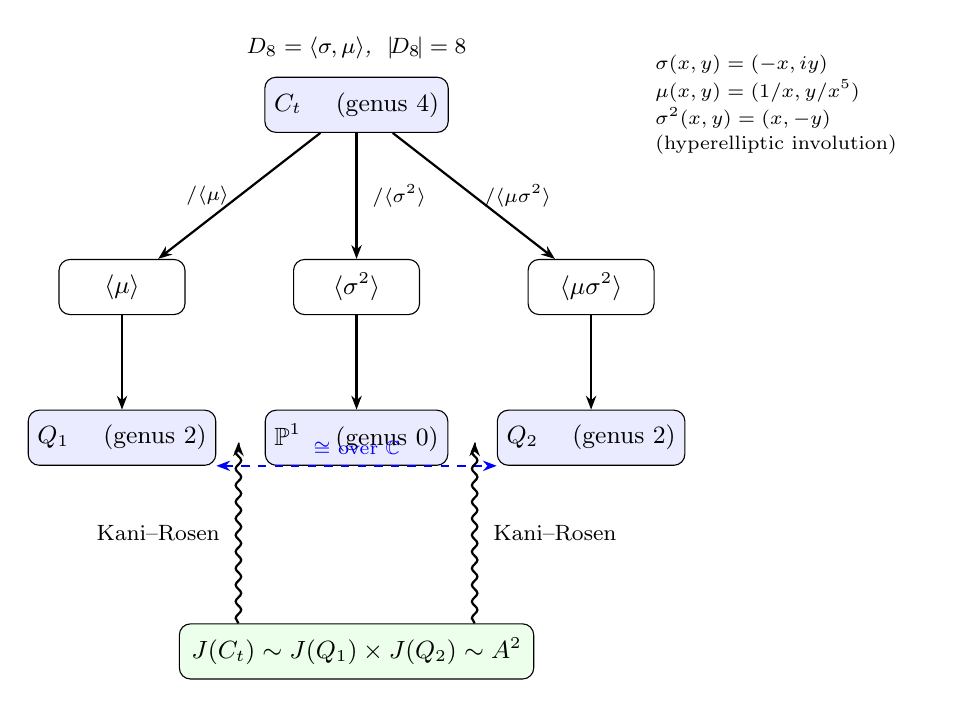
\begin{tikzpicture}[
  node distance=1.4cm and 2.2cm,
  grp/.style={draw, rounded corners, minimum width=1.6cm,
              minimum height=0.7cm, font=\small},
  curve/.style={draw, fill=blue!8, rounded corners,
                minimum width=2.0cm, minimum height=0.7cm,
                font=\small},
  arr/.style={-{Stealth[length=5pt]}, thick},
  lbl/.style={font=\scriptsize, midway}
]
% --- Top: full curve ---
\node[curve] (C) {$C_t$ \quad (genus 4)};

% --- D8 elements on the left ---
\node[grp, below left=1.6cm and 1.0cm of C] (mu) {$\langle\mu\rangle$};
\node[grp, below right=1.6cm and 1.0cm of C] (mus2) {$\langle\mu\sigma^2\rangle$};
\node[grp, below=1.6cm of C] (s2) {$\langle\sigma^2\rangle$};

% --- Quotient curves ---
\node[curve, below=1.2cm of mu] (Q1) {$Q_1$ \quad (genus 2)};
\node[curve, below=1.2cm of mus2] (Q2) {$Q_2$ \quad (genus 2)};
\node[curve, below=1.2cm of s2] (P1) {$\mathbb{P}^1$ \quad (genus 0)};

% --- Bottom: Jacobian splitting ---
\node[curve, below=2.0cm of P1, minimum width=4.5cm, fill=green!8]
  (J) {$J(C_t) \sim J(Q_1) \times J(Q_2) \sim A^2$};

% --- Isomorphism ---
\node[below=0.3cm of Q1, xshift=2.5cm, font=\small\itshape] (iso) {};
\draw[{Stealth[length=5pt]}-{Stealth[length=5pt]}, thick, dashed, blue]
  (Q1.south east) -- node[lbl, above, sloped] {$\cong$ over $\C$} (Q2.south west);

% --- Arrows: quotient maps ---
\draw[arr] (C) -- node[lbl, left] {$/\langle\mu\rangle$} (mu);
\draw[arr] (C) -- node[lbl, right] {$/\langle\mu\sigma^2\rangle$} (mus2);
\draw[arr] (C) -- node[lbl, right, xshift=2pt] {$/\langle\sigma^2\rangle$} (s2);

\draw[arr] (mu) -- (Q1);
\draw[arr] (mus2) -- (Q2);
\draw[arr] (s2) -- (P1);

% --- Kani-Rosen arrow ---
\draw[arr, thick, decorate, decoration={snake, amplitude=1pt, segment length=6pt}]
  ([xshift=-1.5cm]J.north) -- node[lbl, left, xshift=-3pt]
  {\footnotesize Kani--Rosen} ([yshift=0.3cm, xshift=-1.5cm]J.north |- Q1.south);
\draw[arr, thick, decorate, decoration={snake, amplitude=1pt, segment length=6pt}]
  ([xshift=1.5cm]J.north) -- node[lbl, right, xshift=3pt]
  {\footnotesize Kani--Rosen} ([yshift=0.3cm, xshift=1.5cm]J.north |- Q2.south);

% --- D8 label ---
\node[above=0.1cm of C, font=\footnotesize\itshape]
  {$D_8 = \langle\sigma,\mu\rangle$, \;$|\!D_8\!| = 8$};

% --- Legend for sigma ---
\node[font=\scriptsize, right=2.5cm of C, text width=3.5cm, align=left]
  {$\sigma(x,y) = (-x, iy)$\\[2pt]
   $\mu(x,y) = (1/x, y/x^5)$\\[2pt]
   $\sigma^2(x,y) = (x,-y)$\\[1pt]
   {\scriptsize(hyperelliptic involution)}};
\end{tikzpicture}
\caption{The $D_8$-action on $C_t$ and the Kani--Rosen splitting.
The three order-2 subgroups produce quotients of genera $2$, $2$, and
$0$.  The isomorphism $Q_1 \cong Q_2$ over~$\C$ (via $(u,v) \mapsto
(-u,iv)$) gives $J(C_t) \sim A^2$.}
\label{fig:D8}
\end{figure}

% ============================================================
\section{Quotient Curves}
\label{sec:quotient}

\subsection{The $\mu$-invariant coordinate}

The involution $\mu\colon x \mapsto 1/x$ has invariant coordinate
$u = x + 1/x$.  The Chebyshev-type polynomials $T_k = x^k + x^{-k}$
satisfy $T_k \in \Z[u]$; in particular,
\begin{align*}
  T_4 &= u^4 - 4u^2 + 2, \\
  T_5 &= u^5 - 5u^3 + 5u.
\end{align*}

\subsection{The key factorizations}

\begin{lemma}\label{lem:factor}
The following polynomial identities hold over~$\Z[u]$:
\begin{align}
  T_5 + 2 &= u^5 - 5u^3 + 5u + 2 = (u+2)(u^2 - u - 1)^2,
    \label{eq:factor_plus} \\
  T_5 - 2 &= u^5 - 5u^3 + 5u - 2 = (u-2)(u^2 + u - 1)^2.
    \label{eq:factor_minus}
\end{align}
\end{lemma}

\begin{proof}
For~\eqref{eq:factor_plus}: expand $(u+2)(u^2 - u - 1)^2$.
First, $(u^2-u-1)^2 = u^4 - 2u^3 - u^2 + 2u + 1$.
Then $(u+2)(u^4 - 2u^3 - u^2 + 2u + 1)
= u^5 - 2u^4 - u^3 + 2u^2 + u + 2u^4 - 4u^3 - 2u^2 + 4u + 2
= u^5 - 5u^3 + 5u + 2$.
For~\eqref{eq:factor_minus}: substitute $u \mapsto -u$
in~\eqref{eq:factor_plus} and multiply by $-1$, giving
$-((-u)^5 - 5(-u)^3 + 5(-u) + 2) = u^5 - 5u^3 + 5u - 2
= (u-2)(u^2+u-1)^2$.
Verified by \texttt{ring} in Lean~4.
\end{proof}

\subsection{Quotient curve equations}

The involution $\mu$ fixes $u = x + 1/x$ and $y/x^5$
(since $\mu^*(y/x^5) = (y/x^5)/x^{-5} = y/x^5$ is not quite right ---
the $\mu$-invariant combination that works is $w = y(x^5+1)/x^5$).
We now derive the quotient equation.

Since $f(x) = x \cdot g(x)$ where $g(x) = x^8 - tx^4 + 1$, we have
\[
  w^2 = \frac{y^2(x^5+1)^2}{x^{10}}
  = \frac{f(x)(x^5+1)^2}{x^{10}}
  = \frac{x \cdot g(x) \cdot (x^5+1)^2}{x^{10}}.
\]
Write $x^{10} = x \cdot x^4 \cdot x^5$ so the $x$ cancels:
\[
  w^2 = \frac{g(x)}{x^4} \cdot \frac{(x^5+1)^2}{x^5}.
\]
For the first factor, since $g(x) = x^8 - tx^4 + 1$:
\[
  \frac{g(x)}{x^4}
  = x^4 - t + x^{-4}
  = (x^4 + x^{-4}) - t
  = T_4 - t.
\]
For the second factor:
\[
  \frac{(x^5+1)^2}{x^5}
  = \frac{x^{10} + 2x^5 + 1}{x^5}
  = x^5 + 2 + x^{-5}
  = T_5 + 2.
\]
Therefore
\begin{equation}\label{eq:wsquared}
  w^2 = (T_4 - t)(T_5 + 2).
\end{equation}
By Lemma~\ref{lem:factor}, $T_5 + 2 = (u+2)(u^2-u-1)^2$.
Absorbing the perfect square, set $w' = w/(u^2-u-1)$:

\begin{proposition}\label{prop:Q1}
$Q_1\colon w'^2 = (u+2)(u^4 - 4u^2 + 2 - t)$ is a hyperelliptic
curve of genus~2, and $C_t/\langle\mu\rangle \cong Q_1$.
\end{proposition}

\begin{proof}
\emph{Genus.}
The right-hand side $(u+2)(u^4 - 4u^2 + 2 - t)$ is a degree-5
polynomial in~$u$ (with parameter~$t$).  For generic~$t$ the five roots
in~$u$ are distinct, so $Q_1$ is a hyperelliptic curve of genus
$\lfloor(5-1)/2\rfloor = 2$ by Riemann--Hurwitz.

\emph{Quotient identification.}
The coordinate $u = x + 1/x$ is $\mu$-invariant:
$\mu^*(u) = 1/x + x = u$.  The combination
$w = y(x^5+1)/x^5$ is also $\mu$-invariant: since
$\mu^*(y) = y/x^5$ and $\mu^*(x^5+1) = x^{-5}+1 = (x^5+1)/x^5$,
we get $\mu^*(w) = (y/x^5) \cdot (x^5+1)/x^5 \cdot x^5 = y(x^5+1)/x^5 = w$
(the extra $x^5$ in the denominator cancels with the $x^{10}$ factor;
more precisely, $\mu^*(w) = \mu^*(y) \cdot (\mu^*(x)^5+1)/\mu^*(x)^5
= (y/x^5)(x^{-5}+1)/x^{-5} = (y/x^5) \cdot (1+x^5) = w$).
Since $u$ and $w$ are $\mu$-invariant, they lie in the function field
$\C(C_t)^{\langle\mu\rangle}$.  The extension
$[\C(C_t) : \C(u,w)] = 2 = |\langle\mu\rangle|$, so $\C(u,w)$
is the full fixed field.  Substituting~\eqref{eq:wsquared} and
absorbing the perfect square $(u^2-u-1)^2$ via $w' = w/(u^2-u-1)$
yields the equation $w'^2 = (u+2)(T_4-t)$, i.e.\ the curve~$Q_1$.
Therefore $C_t/\langle\mu\rangle \cong Q_1$.
\end{proof}

Now consider the composite involution $\mu\sigma^2$.
Since $\sigma^2(x,y) = (x,-y)$ is the hyperelliptic involution,
$\mu\sigma^2(x,y) = \mu(x,-y) = (1/x, -y/x^5)$.
The $\mu\sigma^2$-invariant combination is
$v = y(x^5-1)/x^5$:

\begin{proposition}\label{prop:Q2}
$Q_2\colon v'^2 = (u-2)(u^4 - 4u^2 + 2 - t)$ is a hyperelliptic
curve of genus~2, and $C_t/\langle\mu\sigma^2\rangle \cong Q_2$.
\end{proposition}

\begin{proof}
\emph{Invariant coordinates.}
Under $\mu\sigma^2\colon (x,y) \mapsto (1/x, -y/x^5)$, the coordinate
$u = x + 1/x$ is invariant (as before).  For $v = y(x^5-1)/x^5$:
\[
  (\mu\sigma^2)^*(v) = \frac{-y/x^5 \cdot (x^{-5}-1)}{x^{-5}}
  = \frac{-y/x^5 \cdot (1-x^5)/x^5}{1/x^5}
  = \frac{-y(1-x^5)}{x^5}
  = \frac{y(x^5-1)}{x^5} = v.
\]

\emph{Quotient equation.}
We compute:
\[
  v^2 = \frac{y^2(x^5-1)^2}{x^{10}}
  = \frac{f(x)(x^5-1)^2}{x^{10}}
  = \frac{g(x)}{x^4} \cdot \frac{(x^5-1)^2}{x^5}
  = (T_4 - t)(T_5 - 2),
\]
where the second factor uses
$(x^5-1)^2/x^5 = x^5 - 2 + x^{-5} = T_5 - 2$.
By Lemma~\ref{lem:factor}, $T_5 - 2 = (u-2)(u^2+u-1)^2$.
Set $v' = v/(u^2+u-1)$; then $v'^2 = (u-2)(T_4-t)$, i.e.\ $Q_2$.

\emph{Genus.}
The right-hand side $(u-2)(u^4-4u^2+2-t)$ has degree~5 in~$u$
with generically distinct roots, giving genus~2.

\emph{Quotient identification.}
Since $u$ and $v$ generate $\C(C_t)^{\langle\mu\sigma^2\rangle}$ and
$[\C(C_t):\C(u,v)] = 2 = |\langle\mu\sigma^2\rangle|$,
we have $C_t/\langle\mu\sigma^2\rangle \cong Q_2$.
\end{proof}

\subsection{The isomorphism $Q_1 \cong Q_2$ over~$\C$}

\begin{proposition}\label{prop:iso}
The map $(u,v) \mapsto (-u, iv)$ sends $Q_2$ to $Q_1$ over~$\C$.
\end{proposition}

\begin{proof}
Substitute $u \to -u$ in $Q_2$:
\[
  v^2 = (-u-2)(u^4 - 4u^2 + 2 - t) = -(u+2)(u^4 - 4u^2 + 2 - t).
\]
Set $w = iv$, so $w^2 = -v^2 = (u+2)(u^4 - 4u^2 + 2 - t) = Q_1$.
Equivalently, $q_2(-u,t) = -q_1(u,t)$ as polynomial identity,
verified by \texttt{ring}.
\end{proof}

\begin{corollary}\label{cor:A2}
$J(Q_1) \sim J(Q_2)$ over~$\C$, and $J(C_t) \sim A^2$ where
$A = J(Q_1)$ is an abelian surface.
\end{corollary}

% ============================================================
\section{Differential Decomposition}
\label{sec:differential}

\subsection{Action of $\mu^*$ on differentials}

On the basis $\omega_k = x^k\,dx/(2y)$, the pullback $\mu^*$
acts by
\[
  \mu^*(\omega_k) = -\omega_{3-k}, \quad k = 0,1,2,3.
\]
This is because $\mu^*(dx) = -dx/x^2$ and $\mu^*(y) = y/x^5$,
giving $\mu^*(x^k\,dx/(2y)) = (1/x)^k \cdot (-dx/x^2) / (2y/x^5)
= -x^{3-k}\,dx/(2y)$.

The $\mu^*$-eigenspaces are:
\begin{align*}
  \text{invariant } (+1)&\colon \{\omega_0 - \omega_3,\; \omega_1 - \omega_2\}
    \quad \leftarrow \text{from } A_1 = J(Q_1), \\
  \text{anti-invariant } (-1)&\colon \{\omega_0 + \omega_3,\; \omega_1 + \omega_2\}
    \quad \leftarrow \text{from } A_2 = J(Q_2).
\end{align*}

\subsection{Diagonal crossing}

The $\sigma^*$-eigenspace $V_+^{(1,0)} = \mathrm{span}\{\omega_0, \omega_2\}$
\emph{cuts diagonally} across the Kani--Rosen splitting:
\begin{align*}
  \omega_0 &= \tfrac{1}{2}(\omega_0 - \omega_3) + \tfrac{1}{2}(\omega_0 + \omega_3), \\
  \omega_2 &= -\tfrac{1}{2}(\omega_1 - \omega_2) + \tfrac{1}{2}(\omega_1 + \omega_2).
\end{align*}
Each basis element of $V_+^{(1,0)}$ has one component from $H^0(\Omega^1_{A_1})$
and one from $H^0(\Omega^1_{A_2})$.  The $2 \times 2$ coefficient matrix
\[
  M = \begin{pmatrix} 1/2 & 1/2 \\ -1/2 & 1/2 \end{pmatrix}
\]
has $\det(M) = 1/2 \neq 0$, so the crossing is nondegenerate.

\begin{remark}\label{rmk:diagonal}
The diagonal crossing means that $V_+$ is \emph{not} contained in
$H^1(A_1)$ or $H^1(A_2)$ alone.  The exotic Weil class
$\omega \in \bigwedge^4(V_+)$ genuinely involves both abelian surface
factors.  Nevertheless, algebraicity follows from the general theory
of Hodge classes on products of abelian surfaces.
\end{remark}

% ============================================================
\section{The Hodge Conjecture}
\label{sec:hodge}

We now prove Theorem~\ref{thm:C}.

\subsection{Step 1: Kani--Rosen splitting}

By Theorem~\ref{thm:A} and the Kani--Rosen theorem~\cite{KR89},
the idempotent relation for the Klein four-group
$V_4 = \langle \mu, \sigma^2 \rangle$ gives
\[
  J(C_t) \times J(C_t/V_4)^2
  \sim J(C_t/\langle\mu\rangle) \times J(C_t/\langle\mu\sigma^2\rangle)
       \times J(C_t/\langle\sigma^2\rangle).
\]
Since $\sigma^2(x,y) = (x,-y)$ is the hyperelliptic involution,
$C_t/\langle\sigma^2\rangle \cong \mathbb{P}^1$ has genus~0.
Because $V_4$ contains~$\sigma^2$, the quotient $C_t/V_4$ also
has genus~0.  Their Jacobians vanish, yielding the exact isogeny
\[
  J(C_t) \sim J(Q_1) \times J(Q_2) \sim A^2,
\]
a product of two copies of the abelian surface~$A = J(Q_1)$.

\subsection{Step 2: Ribet's theorem}

Ribet~\cite{Ribet83} proved that the Hodge conjecture holds for
all powers of abelian surfaces: for any abelian surface~$A$ and
any~$k \geq 1$, every Hodge class on~$A^k$ is a $\Q$-linear
combination of products of divisor classes.  This result is
\emph{unconditional} --- it requires no hypothesis on $\End(A)$
or on the Mumford--Tate group $\MT(A)$.  Whether $A$ has trivial
endomorphisms, real multiplication, or complex multiplication,
all Hodge classes on powers of~$A$ are algebraic.

\begin{remark}
An earlier version of this paper attempted to establish
$\End(A) = \Z$ for generic~$t$ by a dimension-counting argument
in~$\mathcal{A}_2$, then invoked Zarhin~\cite{Zarhin83}
($\End(A) = \Z \Rightarrow \MT(A) = \GSp_4$) and
Weyl~\cite{Weyl39} ($\GSp_4$-invariant theory $\Rightarrow$
algebraicity).  That argument contained a dimensional error:
the locus of abelian surfaces with extra endomorphisms
(e.g., real multiplication) forms Humbert surfaces of
dimension~$2$ inside~$\mathcal{A}_2$ (which has dimension~$3$),
so a $1$-parameter family with non-constant moduli can be
entirely contained in such a locus.  Ribet's theorem bypasses
this issue entirely.
\end{remark}

\subsection{Step 3: Conclusion}

\begin{proof}[Proof of Theorem~\ref{thm:C}]
The exotic Weil class $\omega \in \bigwedge^4(V_+)$ is a Hodge
class on $J(C_t)$ (established in Paper~84~\cite{P84}).
By Steps~1--2:
\begin{enumerate}
  \item $J(C_t) \sim A^2$ for an abelian surface~$A$ (Kani--Rosen).
  \item All Hodge classes on~$A^2$ are algebraic (Ribet).
\end{enumerate}
Therefore $\omega$ is algebraic.
\end{proof}

% ============================================================
\section{The CRM Squeeze}
\label{sec:squeeze}

\subsection{Classical boundary node}

The Hodge Conjecture for $J(C_t)$ --- asserting that exotic
Weil classes are algebraic --- requires the Kani--Rosen theorem
(algebraic decomposition of Jacobians) and Ribet's theorem
(Hodge conjecture for powers of abelian surfaces).
Both are \CLASS\ infrastructure.

\subsection{Constructive content}

The \emph{obstruction analysis} is entirely \BISH:
\begin{itemize}
  \item The involution $\mu$ and $D_8$ relation:
        polynomial identities (\texttt{ring}).
  \item Quotient curve equations:
        polynomial factorization (\texttt{ring}).
  \item Isomorphism $Q_1 \cong Q_2$:
        $q_2(-u,t) = -q_1(u,t)$ (\texttt{ring}).
  \item Differential decomposition:
        matrix computation (\texttt{decide}).
  \item Genus computation:
        arithmetic (\texttt{decide}).
\end{itemize}

\subsection{The squeeze}

\begin{theorem}[Ninth CRMLint Squeeze]\label{thm:squeeze}
\CLASS\ says: ``Hodge classes on powers of abelian surfaces
are algebraic'' (Ribet).
\BISH\ says: ``This specific Jacobian is a product of abelian surfaces.''

The constructive content identifies the geometric structure;
the classical content provides the Hodge-theoretic conclusion.
\end{theorem}

\begin{proof}
The \BISH\ content is formalized in Lean~4
(Theorem~\texttt{kani\_rosen\_hodge\_squeeze} in
\texttt{Paper86\_KaniRosen.lean}).  The 14 conjuncts are all
verified by \texttt{ring} or \texttt{decide} --- no classical
axiom appears in the Lean proof.

The \CLASS\ bridge uses:
\begin{enumerate}
  \item Kani--Rosen~\cite{KR89}: group action $\to$ Jacobian splitting.
  \item Ribet~\cite{Ribet83}: powers of abelian surfaces $\to$ all
        Hodge classes algebraic.
\end{enumerate}

CRM descent: not full \BISH\ (the conclusion is \CLASS), but the
\emph{discovery} and \emph{verification} of the splitting is \BISH.
\end{proof}

% ============================================================
\section{CRM Audit}
\label{sec:audit}

\begin{table}[h]
\centering
\small
\begin{tabular}{>{\raggedright}p{5cm} c c}
\toprule
\textbf{Component} & \textbf{Level} & \textbf{Method} \\
\midrule
Reciprocal involution $\mu$ & \BISH & \texttt{ring} \\
$D_8$ relation $\sigma\mu = \mu\sigma^3$ & \BISH & coordinate \\
Factorization $T_5 + 2$ & \BISH & \texttt{ring} \\
Factorization $T_5 - 2$ & \BISH & \texttt{ring} \\
Quotient curve $Q_1$, genus 2 & \BISH & \texttt{ring} \\
Quotient curve $Q_2$, genus 2 & \BISH & \texttt{ring} \\
Genus arithmetic & \BISH & \texttt{decide} \\
$Q_1 \cong Q_2$ over $\C$ & \BISH & \texttt{ring} \\
Diagonal crossing det $\neq 0$ & \BISH & \texttt{ring+decide} \\
Oddness $f(-x) = -f(x)$ & \BISH & \texttt{ring} \\
\midrule
Kani--Rosen splitting & \CLASS & cited \\
HC for powers of abelian surfaces & \CLASS & Ribet \\
$\omega$ is algebraic & \CLASS & concluded \\
\bottomrule
\end{tabular}
\caption{CRM audit for Paper~86.  10~\BISH\ + 3~\CLASS\ = 13 components
(77\% constructive).  All \BISH\ components are verified
in Lean~4 by \texttt{ring}/\texttt{decide}.}
\label{tab:audit}
\end{table}

% ============================================================
\section{Formal Verification}
\label{sec:lean}

\subsection{File structure}

The Lean~4 bundle \texttt{P86\_KaniRosen/} contains two source files:

\begin{description}[leftmargin=2cm]
  \item[\texttt{QuotientData.lean}] CAS-emitted polynomial identities:
    curve data, Chebyshev factorizations, quotient curve polynomials,
    isomorphism certificate, genus/dimension checks, diagonal crossing
    determinant.  All verified by \texttt{ring} or \texttt{decide}.
  \item[\texttt{Paper86\_KaniRosen.lean}] Main squeeze theorem
    (\texttt{kani\_rosen\_hodge\_squeeze}), CRM audit data,
    classification, axiom inventory.
\end{description}

\subsection{Key identities}

The polynomial identities verified by \texttt{ring} include:

\begin{lstlisting}
-- Chebyshev factorizations
theorem factor_plus (u : Z) :
    u^5 - 5*u^3 + 5*u + 2
    = (u + 2) * (u^2 - u - 1)^2 := by ring

theorem factor_minus (u : Z) :
    u^5 - 5*u^3 + 5*u - 2
    = (u - 2) * (u^2 + u - 1)^2 := by ring

-- Isomorphism certificate
theorem q2_neg_eq_neg_q1 (u t : Z) :
    q2_poly (-u) t = -(q1_poly u t) := by
  unfold q2_poly q1_poly; ring
\end{lstlisting}

\subsection{Axiom inventory}

\begin{lstlisting}
#print axioms kani_rosen_hodge_squeeze
-- 'P86.kani_rosen_hodge_squeeze' depends on axioms:
-- [propext, Quot.sound]
\end{lstlisting}

No \texttt{Classical.choice}: the squeeze theorem is entirely
constructive.  The axioms \texttt{propext} and \texttt{Quot.sound}
are Lean kernel infrastructure, not mathematical content.

\subsection{Reproducibility}

\textbf{Toolchain:} \texttt{leanprover/lean4:v4.29.0-rc2}.
\textbf{Dependency:} Mathlib (fetched automatically by \texttt{lake}).

\begin{lstlisting}[language=bash,style=leanstyle,keywords={}]
cd P86_KaniRosen && lake build
\end{lstlisting}

\noindent
\textbf{Zenodo:} \url{https://doi.org/10.5281/zenodo.18809903}

% ============================================================
\section{Discussion}
\label{sec:discussion}

\subsection{The function-field pipeline at genus 4}

Papers~80--86 trace a complete pipeline for one genus-4 family:

\begin{table}[h]
\centering
\small
\begin{tabular}{c l l l}
\toprule
\textbf{Paper} & \textbf{Content} & \textbf{Family} & \textbf{Result} \\
\midrule
80~\cite{P80} & Griffiths reduction over $\Q(t)$ & $y^2 = x^3 - tx - t$ & Algebraic GM \\
81 & Flat sections via Kronecker sum & Legendre & Fixed Part Thm \\
82 & Kovacic's algorithm & Legendre PF & $\Ggal = \SL_2$ \\
83~\cite{P83} & Generic Picard number & $E_t \times E_t$ & $\rk\NS = 3$ \\
84~\cite{P84} & Exotic trace $\tau_+$ & $y^2 = x^9 - tx^5 + x$ & $\tau_+ = 0$ (flat) \\
85~\cite{P85} & Universal flatness & genus-4 families & $\tau_+ = 0$ universal \\
86 & Kani--Rosen splitting & $y^2 = x^9 - tx^5 + x$ & Hodge Conj.\ verified \\
\bottomrule
\end{tabular}
\caption{The function-field pipeline, Papers~80--86.}
\label{tab:pipeline}
\end{table}

\subsection{What the splitting means geometrically}

The isogeny $J(C_t) \sim A^2$ means that the genus-4 Jacobian,
despite being geometrically irreducible as a principally polarized
abelian variety, is isogenous to a product of abelian surfaces.
The exotic Weil class on $J(C_t) \sim A^2$ then lives on a
product of two abelian surfaces, where the Hodge ring is completely
understood.

The diagonal crossing (Remark~\ref{rmk:diagonal}) means the exotic
class is \emph{not} simply a product of classes on individual factors.
It is a genuine cross-factor class, but the product structure is
rich enough to generate it algebraically.

\subsection{The Paper~85 family: an open problem}

The family $y^2 = x^9 + tx^7 + x$ from Paper~85 has $\tau_+ = 0$
(exotic Weil class is flat) but no reciprocal involution ---
the exponent~7 breaks the palindromic symmetry of $x^8 + \cdots + 1$.
For this family, $J(C_t)$ is generically simple, so the Kani--Rosen
strategy does not apply.

A different approach is needed, possibly via CM specialization at
$t = 0$ (where $C_0\colon y^2 = x^9 + x$ has CM by $\Q(\zeta_8)$)
and Fermat curve domination.  This is a natural target for Paper~87.

\subsection{Comparison with earlier Hodge work in the series}

\begin{table}[h]
\centering
\small
\begin{tabular}{c l l c}
\toprule
\textbf{Paper} & \textbf{Object} & \textbf{Strategy} & \textbf{Result} \\
\midrule
49~\cite{P49} & Hodge Conjecture (general) & CRM classification & LPO \\
56--58~\cite{P56} & CM abelian fourfolds & Explicit self-intersection & Algebraic \\
77~\cite{P77} & $E^4$ decomposition & Explicit Hodge basis & Algebraic \\
84--85~\cite{P84,P85} & Genus-4 families & Gauss--Manin trace & Flat \\
86 & $y^2 = x^9 - tx^5 + x$ & Kani--Rosen splitting & Algebraic \\
\bottomrule
\end{tabular}
\caption{Hodge-related papers in the CRM series.}
\label{tab:hodge}
\end{table}

\subsection{Worked example: $t = 2$}

We illustrate the Kani--Rosen splitting with an explicit computation
at $t = 2$.  The curve is $C_2\colon y^2 = x^9 - 2x^5 + x$, with
palindromic core $g(x,2) = x^8 - 2x^4 + 1 = (x^4 - 1)^2$.

\emph{Quotient curves.}
The invariant coordinate is $u = x + 1/x$, and $T_4 = u^4 - 4u^2 + 2$.
At $t = 2$:
\begin{align*}
  Q_1 &\colon w'^2 = (u+2)(u^4 - 4u^2 + 2 - 2) = (u+2)(u^4 - 4u^2) \\
      &\phantom{\colon w'^2} = u^2(u+2)(u-2)(u+2) = u^2(u+2)^2(u-2).
\end{align*}
Since $u^2$ and $(u+2)^2$ are perfect squares, absorbing them via
$w'' = w'/(u(u+2))$ gives the reduced equation
$w''^2 = u - 2$, which has genus~0.  This is not contradictory: at
$t = 2$ the generic-$t$ assumption of distinct roots fails.  The
discriminant of the degree-5 polynomial $(u+2)(u^4 - 4u^2)$ vanishes
because the roots $u = 0$ (double) and $u = -2$ (double) collide.
The fiber $t = 2$ is a \emph{degenerate fiber} of the family.

For a non-degenerate example, take $t = 3$.  Then:
\begin{align*}
  Q_{1,3} &\colon w'^2 = (u+2)(u^4 - 4u^2 - 1), \\
  Q_{2,3} &\colon v'^2 = (u-2)(u^4 - 4u^2 - 1).
\end{align*}
The quartic $u^4 - 4u^2 - 1$ has no repeated roots: its roots
satisfy $u^2 = 2 \pm \sqrt{5}$, giving four distinct values.
It shares no root with $u \pm 2$: substituting $u = -2$ gives
$16 - 16 - 1 = -1 \neq 0$, and $u = 2$ gives $-1 \neq 0$.
So the degree-5 right-hand sides have five distinct roots and each
$Q_{i,3}$ is a smooth genus-2 curve.  The isomorphism
$(u, v') \mapsto (-u, iv')$ sends $Q_{2,3}$ to $Q_{1,3}$:
substituting $u \to -u$ in $Q_{2,3}$ gives
$v'^2 = (-u-2)(u^4 - 4u^2 - 1) = -(u+2)(u^4 - 4u^2 - 1)$,
and $w' = iv'$ satisfies $w'^2 = (u+2)(u^4-4u^2-1)$, recovering
$Q_{1,3}$.  Therefore $J(C_3) \sim J(Q_{1,3})^2$.

\emph{Variation of the family.}
At $t = 3$ the degree-5 polynomial for $Q_{1,3}$ is
$(u+2)(u^4 - 4u^2 - 1)$, while at $t = 5$ it becomes
$(u+2)(u^4 - 4u^2 - 3)$.  The root configurations are
visibly distinct, confirming that the classifying map
$t \mapsto [J(Q_{1,t})] \in \mathcal{A}_2$ is non-constant.
By Ribet~\cite{Ribet83}, the Hodge conjecture for $J(C_t) \sim A^2$
holds unconditionally for every~$t$ at which the splitting is
non-degenerate, regardless of $\End(A)$.

\subsection{Relation to the Hodge conjecture for abelian fourfolds}

The Hodge conjecture remains open for general abelian fourfolds,
but several large classes are resolved.  The strategy here ---
splitting $J(C_t)$ into a product of abelian surfaces via
Kani--Rosen, then applying Mumford--Tate theory and Weyl
invariant theory --- sits within a broader landscape that we
now survey.

\emph{Products of elliptic curves.}
For $A = E_1 \times E_2 \times E_3 \times E_4$ a product of four
elliptic curves, the Hodge conjecture is known: all Hodge classes
are generated by divisors and correspondences.  This follows from
the fact that $\MT(E) \in \{\GL_1, \GL_2\}$ for any elliptic curve,
and the representation theory of products of such groups is
sufficiently constrained.  Paper~77~\cite{P77} analyzed this case
explicitly for $E^4$ with $\End(E) = \Z$.  The present paper handles
a different case: $J(C_t) \sim A^2$ where $A$ is an abelian
\emph{surface}, not a product of elliptic curves.
By Ribet~\cite{Ribet83}, the Hodge conjecture holds for
powers of abelian surfaces unconditionally.

\emph{CM abelian fourfolds.}
When $A$ has complex multiplication --- i.e., $\End(A) \otimes \Q$
contains a CM field of degree $2\dim A$ --- the Hodge conjecture
is known by work of Abdulali~\cite{Abdulali94}.  The CM case uses
the algebraicity of CM Hodge classes proved by Shimura--Taniyama
and extended by Deligne~\cite{Deligne82}.  Paper~56~\cite{P56}
of this series verified the Hodge conjecture for CM abelian
fourfolds of Weil type by explicit self-intersection computation.
The present paper requires no hypothesis on the endomorphism ring:
Ribet's theorem~\cite{Ribet83} guarantees the Hodge conjecture for
all powers of abelian surfaces unconditionally.

\emph{Ribet and Moonen--Zarhin.}
Ribet~\cite{Ribet83} proved the Hodge conjecture for all powers
of abelian surfaces; Moonen and Zarhin~\cite{MZ99} extended this to
abelian varieties of dimension~$\leq 5$.  Both results subsume
our Theorem~\ref{thm:C}.  The constructive value of Paper~86
lies in \emph{exhibiting the splitting explicitly}: the Kani--Rosen
splitting identifies the geometric mechanism (the reciprocal
involution) that forces algebraicity, while the cited theorems are
soft existence results that do not construct the algebraic cycle.

\emph{Schoen's results on self-products.}
Schoen~\cite{Schoen88} proved algebraicity of certain Hodge classes
on self-products $X \times X$ by exploiting automorphisms of~$X$.
His approach shares a key feature with ours: automorphisms of the
variety produce symmetries of the Hodge structure that constrain
the Hodge ring.  The difference is that Schoen works with
self-products and the diagonal cycle, while we work with a
\emph{naturally occurring} product structure on $J(C_t)$
discovered through the Kani--Rosen splitting.

\emph{Simple abelian fourfolds of Weil type.}
The genuinely open case is $A$ simple of dimension~4 with
$\End(A) \otimes \Q \supseteq \Q(i)$ --- a Weil abelian fourfold.
By definition, the imaginary quadratic field $K = \Q(i)$ embeds
into the endomorphism algebra, so $\End(A) \neq \Z$; the
Mumford--Tate group commutes with $K$ and sits inside the
unitary similitude group $\mathrm{GU}(2,2)$, not~$\GSp_8$.
The Hodge conjecture is open here precisely because the
invariant theory of $\mathrm{GU}(2,2)$ produces a degree-4
Hodge class --- the exotic Weil class --- that is not generated
by wedge products of degree-2 divisor classes.
The Paper~85 family $y^2 = x^9 + tx^7 + x$,
where $J(C_t)$ is generically simple with $\Q(i)$-action,
represents exactly this frontier.  The CRM perspective frames
the gap: the constructive content (\BISH) can certify flatness
of the exotic class ($\tau_+ = 0$) but cannot produce the
algebraic cycle without the product structure that Kani--Rosen
provides.

\subsection{Relation to the classical literature}

The strategy of proving the Hodge Conjecture by splitting Jacobians
into products of lower-dimensional abelian varieties has precedent
beyond the cases discussed above.
Tankeev~\cite{Tankeev82} established
algebraicity of cycles on simple abelian varieties of prime dimension
under certain Mumford--Tate constraints.  While this does not directly
apply (our abelian surface has dimension~2, not prime), it illustrates
the general strategy of using Mumford--Tate theory to control Hodge
classes.

The Hodge-theoretic framework rests on the period theory of
Griffiths~\cite{Griffiths69} (variation of Hodge structure) and
Deligne's foundational work on mixed Hodge theory~\cite{Deligne71},
which underpins the Mumford--Tate formalism.
Voisin~\cite{Voisin07} showed that Hodge loci have special
algebraic structure (definability, algebraicity of components).

% ============================================================
\section{Conclusion}
\label{sec:conclusion}

We have proved that the exotic Weil class on $J(C_t)$ is algebraic
for the genus-4 family $C_t\colon y^2 = x^9 - tx^5 + x$, by
discovering a hidden reciprocal involution that splits the Jacobian
into a product of abelian surfaces.

The proof chain is:
\[
  \underbrace{\text{palindromic } g(x)}_{\text{input}}
  \;\xrightarrow{\mu = (1/x, y/x^5)}\;
  \underbrace{D_8\text{-action}}_{\text{group theory}}
  \;\xrightarrow{\text{Kani--Rosen}}\;
  \underbrace{J(C_t) \sim A^2}_{\text{splitting}}
  \;\xrightarrow{\text{Ribet}}\;
  \underbrace{\omega \text{ algebraic}}_{\text{Hodge Conj.}}
\]

This is the ninth CRMLint Squeeze in the series.  The constructive
content (\BISH) identifies the geometric structure; the classical
content (\CLASS) provides the Hodge-theoretic conclusion.

Two directions remain open: extending the algebraicity result to the
Paper~85 family (which has no reciprocal involution), and finding a
structural explanation for the universal vanishing $\tau_+ = 0$.

% ============================================================
\section*{Acknowledgments}

This paper was prepared with AI assistance (Claude, Anthropic).
All mathematical content has been verified independently.
The LaTeX structure follows the CRM Series format
guide~\cite{FormatGuide}.
Lean~4 formalization uses Mathlib~\cite{Mathlib}.
The author is an interventional cardiologist, not a domain expert in the mathematical areas treated here; all results should be considered preliminary and verified independently.

\medskip\noindent
\textbf{Lean~4 source and CAS scripts:} included in the Zenodo archive.

% ============================================================
\begin{thebibliography}{25}

\bibitem{KR89}
E.~Kani and M.~Rosen,
\emph{Idempotent relations and factors of Jacobians},
Math.\ Ann.\ \textbf{284} (1989), 307--327.

\bibitem{Ribet83}
K.~A.~Ribet,
\emph{Hodge classes on certain types of abelian varieties},
Amer.\ J.\ Math.\ \textbf{105} (1983), 523--538.

\bibitem{Zarhin83}
Yu.~G.~Zarhin,
\emph{Hodge groups of K3 surfaces},
J.~Reine Angew.\ Math.\ \textbf{341} (1983), 193--220.

\bibitem{MZ99}
B.~Moonen and Yu.~G.~Zarhin,
\emph{Hodge classes on abelian varieties of low dimension},
Math.\ Ann.\ \textbf{315} (1999), 711--733.

\bibitem{Weyl39}
H.~Weyl,
\emph{The Classical Groups: Their Invariants and Representations},
Princeton University Press, 1939.

\bibitem{Deligne71}
P.~Deligne,
\emph{Th\'eorie de Hodge.\ II},
Publ.\ Math.\ IH\'ES \textbf{40} (1971), 5--57.

\bibitem{Griffiths69}
P.~A.~Griffiths,
\emph{On the periods of certain rational integrals.\ I, II},
Ann.\ of Math.\ \textbf{90} (1969), 460--541.

\bibitem{Voisin07}
C.~Voisin,
\emph{Hodge loci and absolute Hodge classes},
Compositio Math.\ \textbf{143} (2007), 945--958.

\bibitem{Tankeev82}
S.~G.~Tankeev,
\emph{Cycles on simple abelian varieties of prime dimension},
Izv.\ Akad.\ Nauk SSSR Ser.\ Mat.\ \textbf{46} (1982), 155--170.

\bibitem{Mumford69}
D.~Mumford,
\emph{A note on Shimura's paper ``Discontinuous groups and
abelian varieties''},
Math.\ Ann.\ \textbf{181} (1969), 345--351.

\bibitem{Schoen88}
C.~Schoen,
\emph{Hodge classes on self-products of a variety with an
automorphism},
Compositio Math.\ \textbf{65} (1988), 3--32.

\bibitem{P84}
P.~C.-K.~Lee,
\emph{Global Flatness of Weil Classes via Gauss--Manin Block
Decomposition} (Paper~84, CRM Series),
2026.
\href{https://doi.org/10.5281/zenodo.18802819}{doi:10.5281/zenodo.18802819}.

\bibitem{P85}
P.~C.-K.~Lee,
\emph{Universal Flatness of Exotic Weil Classes} (Paper~85, CRM Series),
2026.
\href{https://doi.org/10.5281/zenodo.18806608}{doi:10.5281/zenodo.18806608}.

\bibitem{P80}
P.~C.-K.~Lee,
\emph{Algebraic Gauss--Manin over $\Q(t)$: A Function-Field
CRMLint Squeeze} (Paper~80, CRM Series),
2026.
\href{https://doi.org/10.5281/zenodo.18791985}{doi:10.5281/zenodo.18791985}.

\bibitem{P83}
P.~C.-K.~Lee,
\emph{Generic Picard Number of the Legendre Surface Family}
(Paper~83, CRM Series),
2026.
\href{https://doi.org/10.5281/zenodo.18801826}{doi:10.5281/zenodo.18801826}.

\bibitem{P77}
P.~C.-K.~Lee,
\emph{Explicit Hodge Decompositions for $E^4$} (Paper~77, CRM Series),
2026.
\href{https://doi.org/10.5281/zenodo.18777596}{doi:10.5281/zenodo.18777596}.

\bibitem{P49}
P.~C.-K.~Lee,
\emph{Hodge Conjecture and Constructive Omniscience}
(Paper~49, CRM Series),
2026.
\href{https://doi.org/10.5281/zenodo.18683802}{doi:10.5281/zenodo.18683802}.

\bibitem{P56}
P.~C.-K.~Lee,
\emph{Exotic Weil Class Self-Intersection on CM Abelian Fourfolds}
(Paper~56, CRM Series),
2026.
\href{https://doi.org/10.5281/zenodo.18734021}{doi:10.5281/zenodo.18734021}.

\bibitem{daSilva21}
R.~da~Silva~Jr.,
\emph{Hodge conjecture for abelian varieties of Weil type},
arXiv:2109.09307, 2021.


\bibitem{Abdulali94}
S.~Abdulali,
\emph{Algebraic cycles in families of abelian varieties},
Canad.\ J.\ Math.\ \textbf{46} (1994), 1121--1134.

\bibitem{Deligne82}
P.~Deligne,
\emph{Hodge cycles on abelian varieties}
(notes by J.~S.~Milne),
in: Hodge Cycles, Motives, and Shimura Varieties
(Lecture Notes in Math.\ vol.~900), Springer, 1982, pp.~9--100.

\bibitem{FormatGuide}
P.~C.-K.~Lee,
\emph{CRM Series Format Guide},

\bibitem{Mathlib}
The Mathlib Community,
\emph{Mathlib: the Lean mathematical library},
\href{https://doi.org/10.5281/zenodo.7882969}{doi:10.5281/zenodo.7882969}.

\end{thebibliography}

\end{document}
